\documentclass[journal]{vgtc}                % final (journal style)
%\documentclass[review,journal]{vgtc}         % review (journal style)
%\documentclass[widereview]{vgtc}             % wide-spaced review
%\documentclass[preprint,journal]{vgtc}       % preprint (journal style)

%% Uncomment one of the lines above depending on where your paper is
%% in the conference process. ``review'' and ``widereview'' are for review
%% submission, ``preprint'' is for pre-publication, and the final version
%% doesn't use a specific qualifier.

%% Please use one of the ``review'' options in combination with the
%% assigned online id (see below) ONLY if your paper uses a double blind
%% review process. Some conferences, like IEEE Vis and InfoVis, have NOT
%% in the past.

%% Please note that the use of figures other than the optional teaser is not permitted on the first page
%% of the journal version.  Figures should begin on the second page and be
%% in CMYK or Grey scale format, otherwise, colour shifting may occur
%% during the printing process.  Papers submitted with figures other than the optional teaser on the
%% first page will be refused. Also, the teaser figure should only have the
%% width of the abstract as the template enforces it.

%% These few lines make a distinction between latex and pdflatex calls and they
%% bring in essential packages for graphics and font handling.
%% Note that due to the \DeclareGraphicsExtensions{} call it is no longer necessary
%% to provide the the path and extension of a graphics file:
%% 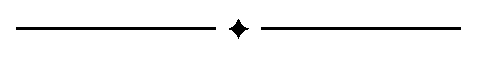
\includegraphics{diamondrule} is completely sufficient.
%%
\ifpdf%                                % if we use pdflatex
  \pdfoutput=1\relax                   % create PDFs from pdfLaTeX
  \pdfcompresslevel=9                  % PDF Compression
  \pdfoptionpdfminorversion=7          % create PDF 1.7
  \ExecuteOptions{pdftex}
  \usepackage{graphicx}                % allow us to embed graphics files
  \DeclareGraphicsExtensions{.pdf,.png,.jpg,.jpeg} % for pdflatex we expect .pdf, .png, or .jpg files
\else%                                 % else we use pure latex
  \ExecuteOptions{dvips}
  \usepackage{graphicx}                % allow us to embed graphics files
  \DeclareGraphicsExtensions{.eps}     % for pure latex we expect eps files
\fi%

%% it is recomended to use ``\autoref{sec:bla}'' instead of ``Fig.~\ref{sec:bla}''
\graphicspath{{figures/}{pictures/}{images/}{./}} % where to search for the images

\usepackage{microtype}                 % use micro-typography (slightly more compact, better to read)
\PassOptionsToPackage{warn}{textcomp}  % to address font issues with \textrightarrow
\usepackage{textcomp}                  % use better special symbols
\usepackage{mathptmx}                  % use matching math font
\usepackage{times}                     % we use Times as the main font
%\renewcommand*\ttdefault{txtt}         % a nicer typewriter font
\usepackage{cite}                      % needed to automatically sort the references
\usepackage{tabu}                      % only used for the table example
\usepackage{booktabs}                  % only used for the table example
%% We encourage the use of mathptmx for consistent usage of times font
%% throughout the proceedings. However, if you encounter conflicts
%% with other math-related packages, you may want to disable it.

%% In preprint mode you may define your own headline.
%\preprinttext{To appear in IEEE Transactions on Visualization and Computer Graphics.}

%% If you are submitting a paper to a conference for review with a double
%% blind reviewing process, please replace the value ``0'' below with your
%% OnlineID. Otherwise, you may safely leave it at ``0''.
\onlineid{0}

%% declare the category of your paper, only shown in review mode
\vgtccategory{Research}
%% please declare the paper type of your paper to help reviewers, only shown in review mode
%% choices:
%% * algorithm/technique
%% * application/design study
%% * evaluation
%% * system
%% * theory/model
\vgtcpapertype{proposal}

%% Paper title.
\title{JuxtaMIDI: Using Data Visualization to Pinpoint Mistakes in MIDI Practice Recordings}

%% This is how authors are specified in the journal style

%% indicate IEEE Member or Student Member in form indicated below
\author{Jeremy Grifski and Stephen Wu}
\authorfooter{
%% insert punctuation at end of each item
\item
 Jeremy Grifski is a student at The Ohio State University. E-mail: grifski.1@osu.edu.
\item
 Stephen Wu is a student at The Ohio State University. E-mail: wu.2719@osu.edu.
}

%other entries to be set up for journal
\shortauthortitle{Biv \MakeLowercase{\textit{et al.}}: Global Illumination for Fun and Profit}
%\shortauthortitle{Firstauthor \MakeLowercase{\textit{et al.}}: Paper Title}

%% Abstract section.
\abstract{
When a musician wants to practice their instrument, they often have to rely
on their peers or an instructor to help them isolate mistakes in their
technique. As an alternative solution, we are proposing a system to answer the
following question: how can we leverage data visualization to pinpoint mistakes
in music data? For the sake of scope, we have chosen to focus on MIDI recordings.
} % end of abstract

%% Keywords that describe your work. Will show as 'Index Terms' in journal
%% please capitalize first letter and insert punctuation after last keyword
\keywords{Music, Data Visualization, MIDI.}

%% ACM Computing Classification System (CCS).
%% See <http://www.acm.org/class/1998/> for details.
%% The ``\CCScat'' command takes four arguments.

\CCScatlist{ % not used in journal version
 \CCScat{K.6.1}{Management of Computing and Information Systems}%
{Project and People Management}{Life Cycle};
 \CCScat{K.7.m}{The Computing Profession}{Miscellaneous}{Ethics}
}

\vgtcinsertpkg

%%%%%%%%%%%%%%%%%%%%%%%%%%%%%%%%%%%%%%%%%%%%%%%%%%%%%%%%%%%%%%%%
%%%%%%%%%%%%%%%%%%%%%% START OF THE PAPER %%%%%%%%%%%%%%%%%%%%%%
%%%%%%%%%%%%%%%%%%%%%%%%%%%%%%%%%%%%%%%%%%%%%%%%%%%%%%%%%%%%%%%%%

\begin{document}

%% the only exception to this rule is the \firstsection command
\firstsection{Introduction and Motivation}

\maketitle

Music is a profession and hobby enjoyed by many people. Unfortunately, the
field hasn't received a lot of attention from the technology community. To
this day, musicians still practice their instruments with little to no
benefit from technology.

One area of music that could really benefit from a technological upgrade would
be practice. After all, practice is usually something that occurs alone without
a lot of feedback. Without access to an instructor, musicians may find it difficult
to self-assess their abilities. They could all benefit from some sort of tool
to help pinpoint their mistakes.

In this project, we built a data visualization dashboard which can be used to
compare practice MIDI files with professional MIDI files. The goal is to isolate
areas in the practice file which are most unlike the professional file for the
sake of improvement.

\section{Related Work}

While there was plenty of motivation for the project, we still needed to
lay the ground work for the project. In particular, we had to come up with some
research questions, design goals, tasks, and metrics which we could use to map
out our implementation.

\subsection{Research Questions}

As mentioned previously, the major research question we looked to address is the
following: how can we leverage data visualization to pinpoint mistakes in MIDI
practice recordings?

Naturally, this question raises several underlying questions such as:

\begin{itemize}
  \item What are practice areas and quantifiable data (pitch, tempo, etc.) that
  we can gleam from MIDI recordings?
  \item What are the most effective ways of visualizing those practice areas?
  \item What are our options in analyzing MIDI files to visualize MIDI events
  in a useful manner for musicians?
  \item How useful is comparing MIDI recordings via velocity, sustain, and note
  frequency over time graphs
  \item Can we algorithmically generate useful automated feedback from analysis
  of these MIDI recordings and graphs
\end{itemize}

In an effort to pinpoint mistakes, we wanted to find the best ways to
represent our musical data, so the user would see value in the tool.

\subsection{Design Goals}

At a high level, our goal was to construct a dashboard split into two panes: the
file pane and the graph pane.

The file pane should contain a list of active MIDI files which are each given a
color for encoding purposes. That means the dashboard should be able to support
about 20 simultaneous MIDI files due to the limits of color perception. This
should be more than enough considering the practicality of comparing that many
recordings.

Each file in the file pane should be able to be selected for viewing purposes
in the graph pane. When unselected, the file's background color should be neutral.
When selected, the file's background color should mirror its color in the graph
pane.

Meanwhile, the graph pane should contain several graphs:

\begin{itemize}
  \item Notes versus Time (master graph)
  \item Notes versus Frequency
  \item Velocity versus Time
  \item Sustain versus Time
\end{itemize}

As a stretch goal, each graph should be connected with the master graph for
filtering purposes. When a section of time is selected in the master graph,
all other graphs should be updated to reflect the new subsection of data. This
would allow a user to hone in on specific mistakes.

In addition, graphs should contain tooltips which will highlight areas with
the highest amount of mistakes. These tooltips should include high level notes
to assist the user in understanding the data.

Finally, the dashboard should be extended to include realtime recording and sheet
music comparison.

\subsection{Tasks and Metrics}

In order to verify the success of the project, we tracked several tasks in
GitHub:

\begin{itemize}
  \item MIDI File Upload
  \item MIDI File Pane
  \item Notes versus Time Graph
  \item Notes versus Frequency Graph
  \item Velocity versus Time Graph
  \item Sustain versus Time Graph
  \item Mistake Analysis for Tooltips
  \item Realtime Recording
  \item Sheet Music Rendering and Comparison
\end{itemize}

Each of these tasks were broken down into smaller tasks as they all need to be
designed, prototyped, and tested.

As for verifying that our design is good, we tested it on users of varying musical
abilities. For less experienced individuals, we had them watch us interact with
the tool through a demonstration where we collected feedback. For experienced
musicians, we had them play a song to generate a MIDI file, then we asked them
to indicate any mistakes they felt they made. Finally, we compared their
personal insight to the tool.

\subsection{Implementation}

Ultimately, JustaMIDI ended up being a web-based tool built entirely as a
static website using just JavaScript, CSS, and HTML.

\subsubsection{Dashboard Overview}

In terms of general design, we went with a dashboard approach using CSS grids.
In other words, we divided the space into four columns by percentage of screen
width from left to right: 9\%, 43\%, 43\%, and 3\%. Likewise, we divided
the space into two rows by screen height from top to bottom: 60\% and auto.

Each dashboard element was then assigned some range of grid points that they
could occupy. For example, the MIDI selection interface was given the entire
first column. Likewise, the pane selection interface was given the entire
last column. Meanwhile, the note graph was given the center two columns of
the top row while the remaining graphs split the bottom row of the same
columns.

\subsubsection{MIDI Selection Interface}

As mentioned, the entire first column was dedicated to the MIDI selection
interface. This interface consisted of a single MIDI upload button and any
number of MIDI file items.

The upload button works just like any file upload interface. When a file is
uploaded, a callback function is executed. In this case, we parse the midi file,
and pass that data to the respective graphs panes to be rendered. At the same
time, we generate a MIDI file list item which allows us to interact with the
loaded file in various ways such as:

\begin{itemize}
  \item Changing its name
  \item Toggling it on/off
  \item Deleting it
  \item Playing/pausing it
\end{itemize}

In addition, it is at this point that we assign the file a color for encoding
purposes in each graph. To aid in encoding, we color the background of the
file element, so it matches any data associated with the file in the various
graph panes.

\subsubsection{Notes Over Time Pane}

In the top pane, we render the notes over time graph. Each note is encoded in
three visual channels: color, position, size. The color gives us the track
mapping, so it should match whatever color the file was assigned in the MIDI
selection pane. Meanwhile, the position encodes two pieces of information:
note and time. Finally, the size encodes note duration.

When looking at this graph, it is helpful to imagine a piano along the y-axis.
Lower pitches are near the top of the graph while higher pitches are closer to the
bottom of the graph. Meanwhile, the x-axis gives us the duration of each note
from the time it begins to the time it ends. Time is given as generic time units
which gain meaning given a tempo. Finally, each note has a tooltip which gives
information like note, start time, duration, and velocity.

To generate these features, we use a combination of open-source libraries, but
the primary tool is D3 which allows us to create graphs from Scalar Vector
Graphics (SVG). In particular, the notes over time graph is generated by
extracting the note information from all active MIDI files and plotting the
results against the axes as rectangles with the appropriate color.

\subsubsection{Note Frequency Pane}

In the bottom left pane, we render the note frequency graph. Here, we filter
the MIDI file data, so we end up with a collection of notes. Each note
corresponds to a number which we dynamically map to their respective letters
using a lookup table (LUT). Using this mapping, we're able to generate a
histogram of notes.

Just like the notes over time plot, we also use D3 here to handle the bulk of
the heavy lifting. At a high level, we use the note counts to plot rectangle
against two axes: frequency and note. The frequency axis is scaled by the
maximum note frequency over all active tracks. Meanwhile, the x-axis
contains a direct mapping of all unique notes over all active tracks. We then
sort that axis by the note frequency of the primary track.

\subsubsection{Note Velocity Pane}

While the other two plots were relatively straightforward, we had a lot of
trouble deciding on the note velocity plot. Ideally, what we would like to be
able to capture in this plot is dynamics. In other words, how can we show
the ebb and flow of volume over time to the user. As it turns out, it is harder
than it seems.

Initially, we tried summing the velocity of all the notes at each time step and
plotting the results. Unfortunately, the resulting curve was pretty eratic. In
fact, we noticed we few bizarre artifacts in the results like a downward
slope over time which didn't make a lot of sense for a nearly constant
volume song. Fortunately, someone pointed out that summing the velocities at
each time step is bad practice because we aren't guaranteed to have the same
number of key presses at any given time. In other words, the maximum volume
is entirely dependent on the maximum number of keys played simultaneously.

To accomodate for this problem, we decided to try plotting the velocity range
over time. The result contains two lines for each track where the space in
between is colored based on the file color. As expected, the x-axis is in the
same units as the notes over time plot, and the y-axis is raw velocity.

\subsubsection{Plot Filtering Pane}

Finally, we added a plot filtering pane which gives us control over which pane
we can see at any given time. There are four options:

\begin{itemize}
  \item All panes as described in the dashboard overview
  \item The notes over time pane alone
  \item The note frequency pane alone
  \item The note velocity over time pane alone
\end{itemize}

When a pane is selected alone, we fill the entire center two columns with that
pane. For example, selecting the note frequency pane makes the other two graph
panes disappear while the note frequency pane is expanded to fill the space.

\subsubsection{Interactivity}

Most of the interactivity elements are in the MIDI selection pane. However, we
haven't discussed exactly how that interactivity works up to this point. To
reiterate, there are four main ways to interact with each file: toggling,
renaming, deleting, and playing.

When we toggle a file, the state of that file changes based on its previous
state. In other words, if we were originally showing a file in all three graphs,
toggling it would remove it from the graphs. Toggling it again would render in
all three graphs once again. Meanwhile, deleting a file will remove the file
from the program completely, and renaming a file updates all the tooltips.

In addition, users can play each file as well. When a file is playing, a marker
is added to each time-domain graph (i.e. notes of time, velocity over time, etc.)
along the x-axis. In addition, the marker is encoded with the color of the
track currently playing. This is all handled through a callback function that
hooks into the MIDI playback utility.

Likewise, users are able to filter by which graph they want to see as mentioned
previously in the Plot Filtering Pane section. Finally, there are a few minor
interactivity features like the ability to scroll along the x-axis of the
time-domain graphs and the ability to hover over graph elements to show tooltips.

\subsection{Environments}

To complete this project, we required the following software:

\begin{itemize}
  \item JavaScript: a web-based programming language
  \item D3.js: a data visualization library
  \item MIDI.js: a MIDI processing library
  \item GarageBand: a MIDI editing tool
  \item GitHub: a version control and project management tool
  \item Travis CI: a continuous integration tool for testing
\end{itemize}

With this software, we were able to build and test the entire system.

\section{Design Method}

Now that we have had the chance to discuss the background and related work,
let's talk about our design choices and how we believe they effectively
accomplish our tasks.

\subsection{Data Abstraction}

For our project, we were working with MIDI files which are event-based music
files. In other words, we were not dealing with audio signals. Instead, we took
a file format which stores music information like tracks, notes, velocities, and
durations, and made sense of it visually.

Despite the fact that the MIDI file format already abstracts music signals,
there still is a case to make to further abstract the data. For example,
MIDI files are entirely in binary which means that they are not easy to read
as a user. As a result, we used a utility to parse the MIDI file into a
JavaScript object.

While the object itself was a bit easier to work with, the data still wasn't
meaningful to our end user. For example, the resulting JavaScript object
contained a lot of nested information about tracks and events but almost no
clear information on how that data maps to musical notes, rhythms, and dynamics.
To make matters worse, MIDI files store events using numeric codes, so the
data is not easy to read. For example, how are we supposed to know what
the following means:

\begin{itemize}
  \item Type: 9
  \item Note: 47
  \item Velocity: (47, 0)
\end{itemize}

\section{Results and Analysis}

Evaluation was done in two phases, an initial prototype on March 7, 2019 and an
updated prototype on April 6, 2019. Feedback was gathered from both phases to
evaluate and improve the product.

For the updated prototype evaluation, we shared the tool with one of our advisors.
Unfortunately, they hadn’t gotten around to the tool in time due to vis paper
deadlines. As a result, we decided to review the tool ourselves.

\subsection{Prototype Design}

The initial prototype aimed to accomplish several of the major tasks mentioned
previously. In particular, the following tasks were implemented:

\begin{itemize}
  \item MIDI File Upload
  \item MIDI File Pane
  \item Notes versus Time Graph
  \item Notes versus Frequency Graph
  \item Velocity versus Time Graph
\end{itemize}

In addition, we added a few extra interactivity features during our own
iterative process:

\begin{itemize}
  \item MIDI File Color Mapping
  \item MIDI File Playback
  \item MIDI File Renaming
  \item MIDI File Toggling
\end{itemize}

With the prototype read to go, we began the evaluation process by presenting
it to the class.

\subsection{Peer Feedback}

In general, feedback was positive. However, there were a few things
that needed improvement in the original prototype. The following
list contains the feedback from our peers:

\begin{itemize}
  \item Colors
  \begin{itemize}
    \item Too closely related (light blue and dark blue)
    \item Yet, calming
  \end{itemize}
  \item Velocity plot
  \begin{itemize}
    \item Difficult to see differences in curves
    \item Plot may not be capturing appropriate data (summing velocities)
    \item Look into normalization
  \end{itemize}
  \item Target audience
  \begin{itemize}
    \item Musicians don't care about time steps - they want beats and measures
  \end{itemize}
  \item Interactivity
  \begin{itemize}
    \item Playback should animate graphs
  \end{itemize}
\end{itemize}

\subsection{Musician Feedback}

In addition to the in class feedback, we also chose to evaluate the JuxtaMIDI
platform ourselves. In particular, Stephen leveraged his intermediate piano
playing abilities to generate the following list of comments:

\begin{itemize}
  \item Inherent limitations:
  \begin{itemize}
    \item Online, generated MIDI files are often lacking when compared to an
    actual song:
    \begin{itemize}
      \item Song may have a constant velocity for every note.
      \item Key signatures, tempo, and sustain may be missing.
    \end{itemize}
    \item Recorded MIDI files have some of these issues and more:
    \begin{itemize}
      \item Velocity is obtained, but this is not exactly reflective of playing
      on an acoustic piano, which is what would be typically used in performance.
      Keyboards, especially cheaper ones, are simply less expressive than acoustic
      pianos.
      \item If the user is off-time by even a beat, the whole song gets offset.
      If the user corrects their time and becomes on-time, this issue is resolved.
      This means the user needs to be playing to a metronome and correct any time
      lost, which adds additional requirements on their playing.
    \end{itemize}
    \item Preprocessing:
    \begin{itemize}
      \item Key signatures and tempo need to be manually added if needed for tool
      (it isn’t in the current stage).
      \item The MIDI file also needs to be edited to remove any wait in the
      beginning.
    \end{itemize}
  \end{itemize}
  \item Benefits:
  \begin{itemize}
    \item Where this tool thrives is helping identify insights that can’t be
    simply heard or seen in a recording.
    \item Users can upload and play their recordings.
    \item The velocity curve is probably the most novel item, since other tools
    (like GarageBand) provide the features of the Master Note graph.
    \begin{itemize}
      \item Users can follow the sheet music and quickly see how they played
      different sections, e.g. if they played one forte section louder than
      another, or if they mistakenly played one forte section as piano.
    \end{itemize}
  \end{itemize}
  \item Potential:
  \begin{itemize}
    \item This tool would greatly benefit from adding measure count. Since sheet
    music often comes with measure numbers, users could cross-reference their
    playing with the measure number.
    \item Exploring and solving the tempo offset issue would make this tool much
    more useful.
    \item Some additional outlier detection or analysis would also help.
    \item Since musicians are used to sheet music, having a sheet music overlay
    with different colored notes per track would be immensely helpful.
    \begin{itemize}
      \item This would require key signature, tempo, and a really good sheet music generator
    \end{itemize}
  \end{itemize}
\end{itemize}

\subsection{Design Changes}

To address some of the feedback, we decided to look into the
following changes:

\begin{enumerate}
  \item Adding a time marker to show where the user is in the song
  \item Changing velocity plot to be more expressive
  \item Reordering the color array so additional tracks have drastically different colors
  \item Adding option for user to specify tempo, changing time to measure
\end{enumerate}

For the final implementation, we completed \#1 and \#2 for the updated prototype.

\subsection{Production Implementation}

Ultimately, the final production dashboard was extended to include a marker
to illustrate playback. The marker is colored based on which track was playing.

\section{Discussion}

\section{Conclusion}

It may seem odd to want to think of music in a visual way, but we feel our
system will have a positive impact on musicians who want to improve their
practice sessions.

\end{document}
